%!TEX root = 16-ra-letter-NMPCWalkGen.tex
%\newcommand*\refeq[1]{#1}
%\newcommand*\rfrac[2]{{}^{#1}\!/_{#2}}

\section{Derivation of the dynamics}
\label{Sec:dynamic}

In this work the well known Linear Inverted Pendulum Model (LIPM) from \cite{Kajita:icra:2003} is used as the template model of the robot's dynamics 
and the following assumptions are made:
1) the angular momentum produced by the rotations of all the robot parts is supposed to be zero,
2) the robot CoM evolves on a horizontal plane,
3) the normals of the contact forces have to be collinear.
As a consequence, each quantity can be expressed as a function of three degrees of freedom (DoFs), which are the projection of the robot CoM $(x,y)$-position on the ground plane and its free-flyer orientation $\theta$ around the vertical axis $z$.
The reader is kindly referred to \cite{herdt:iros:2010} for a detailed description of the several terms omitted for a sake of clarity in the following section.

\subsection{Discretization of CoM dynamics}
\label{SubSec:comDiscr}

In order to obtain a smooth trajectory, one controls the robot CoM through its jerk $\dddot{c}^{\nu}$ on a preview horizon, where $c$ denotes the position of the CoM in the world frame and $\nu \in \{ x, y \}$
%\footnote{In this algorithm the CoM height is constant, i.e. ${c}^{z}\equiv const.$}
is used to simplify the notation.
This is done by applying a constant sampling period $T$ and by assuming a piecewise constant jerk on each interval, i.e. $\dddot{c}_{k}^{\nu}(t) \equiv constant$, $t \in \left[k T, (k+1) T \right]$, $k\in\{0, 1, ..., N\}$, where $N$ is the length of the preview horizon.

The following time-stepping scheme maps the current state of the frame $c_k^{\nu}$ to the future states by
\begin{equation}
  \label{eq:com_der}
  \hat{c}_{k+j}^{\nu} = A^j \, \hat{c}_{k}^{\nu} \;+\; \sum_{i=0}^{j-1}{A^{i}\,B\,
  \dddot{c}^{\nu}_{k+i}}
  \,\,\, , \,\,\, j \in [0,N] ,
\end{equation}
\vspace*{-0.24cm}
\begin{equation}%\scriptstyle
\label{eq:time_scheme}
    \hat{c}_{k}^{\nu} =
    \begin{bmatrix}
        c_{k}^\nu \\
        \dot c_{k}^\nu\\
        \ddot c_{k}^\nu
    \end{bmatrix},\
    A =
    \begin{bmatrix}
        1 & T & \rfrac{T^2}{2} \\
        0 & 1 & T \\
        0 & 0 & 1
    \end{bmatrix},\
    B =
    \begin{bmatrix}
        \rfrac{T^3}{6} \\
        \rfrac{T^2}{2} \\
        T
    \end{bmatrix}.
\end{equation}
To express the CoM over the preview horizon the vector $C_{k+1}^\nu$ of size $\mathcal{R}^N$ and its derivatives are defined as
\begin{align}
  &C_{k+1}^\nu =
  \begin{bmatrix}
    c_{k+1}^\nu &
    \hdots &
    c_{k+N}^\nu \notag
  \end{bmatrix}^T
  ,
\;%\\
  &\dot{C}_{k+1}^\nu =
  \begin{bmatrix}
    \dot{c}_{k+1}^\nu &
    \hdots &
    \dot{c}_{k+N}^\nu \notag
  \end{bmatrix}^T
  ,
\\
  &\ddot{C}_{k+1}^\nu =
  \begin{bmatrix}
    \ddot{c}_{k+1}^\nu &
    \hdots &
    \ddot{c}_{k+N}^\nu \notag
  \end{bmatrix}^T
  ,
\;%\\
 &\dddot{C}_{k+1}^\nu =
  \begin{bmatrix}
    \dddot{c}_{k+1}^\nu &
    \hdots &
    \dddot{c}_{k+N}^\nu \notag
  \end{bmatrix}^T
  .
\end{align}
Using eq.~(\ref{eq:com_der}), the above vectors can be expressed as a function of the initial state $\hat{c}_k^\nu$ and the CoM jerk
$
\dddot{C}_{k+1}^\nu
%=
  % \begin{bmatrix}
  %   \dddot{c}_{k+1}^\nu &
  %   \hdots &
  %   \dddot{c}_{k+N}^\nu \notag
  % \end{bmatrix}^T
$.
The latter belongs to the free-variable vector of the optimization problem described in section~\ref{Sec:nmpc}.

\subsection{Linear inverted pendulum dynamics}
\label{SubSec:LIPM}

In this chapter the balance criteria used is the one that have the center of pressure (CoP) in the convex hull of the robot's support polygon, which is defined by the contacts with the ground
\cite{Kajita:icra:2003} (see Sec.~\ref{SubSec:constraints}).
Hence, the CoP has to be expressed in terms of the system's free variables, i.e. the CoM jerk.
Using the assumptions made in the introduction of Sec.~\ref{Sec:dynamic}, the robot CoP can be expressed as a linear function of the CoM, i.e.
\begin{equation*}
    z_{k+n}^{\nu} =
    \begin{bmatrix}
        1 & 0 & -\rfrac{h}{g}
    \end{bmatrix} \hat{c}_{k+n}^\nu
    \, , \,\,\, \nu \in \left\{ x,y \right\}
    , n \in [0,N-1]
    ,
\end{equation*}
with $h=c^z-z^z$ being the height of the CoM with respect to the ground and $g$ the norm of the gravity vector.
Using eq.~\eqref{eq:com_der}, a recursive expression for the future evolution of the CoP for a fixed horizon of $N$ sampling steps  is given by
\begin{equation}
    \label{eq:zmp_horizon}
   	z_{k+n}^{\nu} =
   	\begin{bmatrix}
        1 & 0 & -\rfrac{h}{g}
    \end{bmatrix} \left[ A^n \, \hat{c}_{k}^{\nu} \;+\; \sum_{i=0}^{n-1}{A^{i}\,B\,
  \dddot{c}^{\nu}_{k+i}} \right]
  .
\end{equation}
As in Sec.~\ref{SubSec:comDiscr}, the vector
$	Z_{k+1}^\nu =
    \begin{bmatrix}
        z_{k+1}^\nu &
        \hdots &
        z_{k+n}^\nu \notag
  \end{bmatrix}^T$~,
of size $\mathcal{R}^N$, is used to describe the CoP on the preview horizon.
This vector can then be expressed in terms of $\hat{c}_k^\nu$
and $\dddot{C}_{k+1}^\nu$.

\subsection{Automatic foot step placement}
\label{SubSec:automaticFootPlacement}

The adaptive placement of the feet, with the aim to ensure balance of the robot even under external perturbations, is a key-feature of the algorithm.
To this end, consider a frame $\mathcal F$ attached to the support foot, with its current position and orientation on the ground given by $f_k^\eta$, with $\eta \in \{x,y,\theta\}$.
The future steps, also free variable of the optimization problem, are denoted by
\begin{align}
&F_{k+1}^\eta =
    \begin{bmatrix}
        f^\eta_{k+1} &
        f^\eta_{k+2} &
        \hdots &
        f^\eta_{k+N}         	
    \end{bmatrix}^T
    \notag \\
    	\label{eq:Fkp1}
&F_{k+1}^\eta = v_{k+1} f_{k}^{\eta} + V_{k+1} \tilde{F}_{k+1}^{\eta}
\end{align}
with $F_{k+1}^\eta$ of size $\mathcal{R}^N$ representing the foot support position at each time step and $\tilde{F}_{k+1}^\eta$ of size $\mathcal{R}^{nf}$ the actual free variables of the problem.
The vector $v_{k+1} \in \R^N$ and matrix $V_{k+1} \in \R^{N\times nf}$ indicate which step falls in which sampling interval (see \cite{herdt:iros:2010} for more details).
Sampling times correspond to rows, steps to columns, and $nf$ is the maximum number of double support phases in the preview.

In theory, the usage of a single point mass as model prevents the definition of an orientation.
In \cite{herdt:iros:2010} a frame attached to the center mass is defined and the orientation of this frame and the feet directions are optimized.
In this work only the foot step orientations are optimized, and the orientation of the robot free-flyer is computed from this solution.
Let $\text{ff}^{\theta}(t)$, $f^{\theta,L}(t)$ and $f^{\theta,R}(t)$ be respectively the orientation of the free-flyer, the left foot and the right foot at any time $t$.
Hence $\text{ff}^{\theta}(t)$ is by convention :
\begin{align*}
\begin{bmatrix}
	\text{ff}^{\theta}(t) \\
	\dot{\text{ff}}^{\theta}(t) \\
	\ddot{\text{ff}}^{\theta}(t)
\end{bmatrix}
=
\begin{bmatrix}
	\frac{1}{2}(f^{\theta,L}(t)        + f^{\theta,R}(t)) \\
	\frac{1}{2}(\dot{f}^{\theta,L}(t)  + \dot{f}^{\theta,R}(t)) \\
	\frac{1}{2}(\ddot{f}^{\theta,L}(t) + \ddot{f}^{\theta,R}(t))
\end{bmatrix}
.
\end{align*}

%%%%%%%%%%%%%%%%%%%%%%%%%%%%%%%%%%%%%%%%%%%%%%%%%%%%%%%%%%%%%%%%%%%%%%%%%%%%%%%%%%%%%%%%%%%%%%%%%%%%%%%%%%%%%%%%%%%%%%%%%%%%%%%%%%%%%%%%%%%%%%%%%%%%%%%%%%%%%%%%%%%%%%%%%%%%%%%%%%%%%%%%%%%%%%

\section{Nonlinear Model Predictive Control}
\label{Sec:nmpc}

Solving the orientation problem separately from the position problem is a workaround to linearize the CoP (eq.~\eqref{eq:zmpCanonicConstraint}) and foot position (eq.~\eqref{eq:footCanonicConstraint}) constraints derived below.
However, computing separately the orientation and then injecting the solution into the position QP amounts to solve a different problem than the nonlinear combination of both.
In the following the nonlinear problem will be derived and analyzed, and an appropriate approach allowing the real-time execution of the algorithm on the robot will be proposed.

\subsection{The controller}
\label{SubSec:controller}

\begin{figure}[h]
    \centering
    %!TEX root = ../../14-icra-RealTimeNMPC.tex

\tikzstyle{block} = [draw, fill=blue!20, rectangle,
    minimum height=2em, minimum width=5em, align=center]
\tikzstyle{sum} = [draw, fill=blue!20, circle, node distance=1cm]
\tikzstyle{input} = [coordinate]
\tikzstyle{output} = [coordinate]
\tikzstyle{pinstyle} = [pin edge={to-,thin,black}]

% The block diagram code is probably more verbose than necessary
\begin{tikzpicture}[auto, node distance=2cm,>=latex]

    % We start by placing the blocks
    \node [input]  at (0.0, 0.0) (input)  {};
    \node [input]  at (3, 0.0) (velocity) {};
    \node [input]  at (0.2, -2.8) (feedback)  {};
    \node [input]  at (16, -2.8) (feedback2)  {};
    \node []    at ( 0.0, 0.0) (sumin)  {};
    %\node [output]    at ( 15, 0.0) (sumout) {};
    \draw [fill=green,opacity=.2,text opacity=1] (3.5,1.5) rectangle (11.5,-2.7);
    \node at(10,-1.7) {\textcolor{green!20!black!100}{Stack of Task}};

    \node [block] at (4.6,-1.7) (lwc) {
        Left Wrist\\
        Hybrid\\
        Controller        
    };

    \node [block] at (1.7,0.0) (walking) {
        Walking \\
        Task    
    };

    \node [block] at (4.6,0) (wpg) {
        Walking\\
        Pattern\\
        Generator
    };
%    \node [block] at (4.2,0) (dyn) {
%        Dynamic\\
%        Filter
%    };
    \node [block] at (7.5,0) (ttt) {
        Task for\\
        Trajectory\\
        Tracking
    };
    
    \node [block] at (10.5,0) (qp) {
        QP\\
        solver
    };

    \node [block] at (14.0, 0) (system) {
    		Robot Hardware\\
    		{\footnotesize Simulation/Robot}\\
    		and\\
    		{\footnotesize motion capture system}
    	};

    % PATHS
    	% Forward chaine
    \draw [draw,-] (input) -- node {\small ${\mathbf{p}}^{\,{\text {ref}}}$} (walking);
    
    \draw [draw,->] (walking) -- node {\small ${\mathbf v}^{\,{\text{ref}}}$} (wpg);
%    \draw [draw,- ] (walking) -- node {} (velocity);
    \draw [draw,->] (velocity) |- node {} (lwc);
%    \draw [->] (wpg) -- node {\small $c^{ref},f^{ref}$} (dyn);
%    \draw [->] (dyn) -- node {\small $\tilde{c}^{\,ref},f^{ref}$} (sot);
    \draw [->] (wpg) -- node [text width=0.8cm]{\small ${\mathbf{p}_c}^{\,{\text {ref}}}$ ${\mathbf{p}_f}^{\,{\text {ref}}}$} (ttt);
    \draw [->] (ttt) -- node [text width=0.8cm]{
    \small Tasks
    } (qp);
    \draw [->] (qp) -- node [text width=0.6cm]{\small ${\mathbf q}^{\,{\text{ref}}}$ $\dot{{\mathbf q}}^{\,{\text{ref}}}$} (system);
    
    \draw [->] (lwc) -| node [near start, above]{\small ${\mathbf{p}_{lw}}^{\,{\text {ref}}}$} (ttt);
    %\draw [->] (system) -- node {} (sumout);

    % Feedback chaine
%    \draw [- ] (dyn)      -| node {} (feedback);
%    \draw [->] (feedback) -| node {} (wpg);
    
    \draw [- ] (system.east)    -| node {} (feedback2);
    \draw [- ] (feedback2)  -- node [above]{\small $\mathbf{f}_{lw},\mathbf{p}_{w},\mathbf{p}_{lw},\mathbf{p}_{f}$} (feedback);
    \draw [->] (3.0,-2.8) |- node [near start, above]{} ([yshift=-0.2cm]lwc.west);
    \draw [->] (feedback) |- node [below=0.7cm, right]{\small $\mathbf{p}_{ch}$} ([yshift=-0.2cm]walking);

%    \draw [->] (dyn) -| node[above right] {\small $\hat{c}^{\,x,y,\theta}$, $\hat{f}^{\,\,x,y,\theta}$} (wpg);
\end{tikzpicture}
\caption[Control scheme for pulling a stiff hose]{This scheme describe the feedback loop used to control the humanoid robot HRP-$2$. With ${\mathbf{p}}^{\,{\text {ref}}}$ as the user defined pose, ${\mathbf{v}}^{\,{\text {ref}}}$ as the velocity computed from the walking task, ${\mathbf{p}_c}^{\,{\text {ref}}}$ as the center of mass reference trajectory, ${\mathbf{p}_f}^{\,{\text {ref}}}$ as the feet reference trajectories, ${\mathbf q}^{\,{\text{ref}}},\dot{{\mathbf q}}^{\,{\text{ref}}}$ being respectively the generalized position and velocity vector, ${\mathbf{p}_{lw}}^{\,{\text {ref}}}$ as the reference left wrist position, $\mathbf{f}_{lw},\mathbf{p}_{w},\mathbf{p}_{lw},\mathbf{p}_{f},\mathbf{p}_{ch}$ being respectively the measures of the left wrist force sensor, the waist position, the left wrist position, the feet position and the chest position.}

    \caption[Control scheme]{The control scheme: ${Vel}^{\,ref}$ is the input velocity.
     $c^{ref}$ and $f^{ref}$ are respectively the CoM and the feet 3D trajectories
     $\tilde{c}^{\,ref}$ is the CoM trajectory filtered.
     $q^{ref}$, $\dot q^{ref}$ denote respectively the generalized coordinate vector and its derivation.
     }
    \label{fig:combined_feedback_scheme}
\end{figure}

A scheme of the controller is shown in Fig.~\ref{fig:combined_feedback_scheme}.
This open-loop controller is used for tracking respectively a referenced linear and angular velocity.
In the first step, the walking pattern generator (WPG) computes the foot steps and CoM jerk from the given velocity
$ {Vel}^{\,ref}_{k+1} =$~$
\begin{bmatrix}
{Vel}_{k+1}^{x,ref} & {Vel}_{k+1}^{y,ref} & {Vel}_{k+1}^{\theta,ref}
\end{bmatrix} $.
Then it uses an Euler integration scheme to compute the CoM trajectory from its jerk and polynomials of fifth order to retrieve 3D trajectories for the feet from the foot step planning.
The CoM computed by the WPG is then filtered (see Sec.~\ref{Sec:dynamic_filter}) and sent altogether with the feet trajectory to a generalized inverse kinematics algorithm.
The output is a whole-body walking trajectory that can be applied directly on the robot.
The WPG is then reinitialized with the current reference velocity input and with the corrected initial states of the dynamic filter.

\subsection{The cost function}
\label{SubSec:costFunction}

The cost function used in the NMPC is given by
\begin{equation}
    \min_{U_{k}} \frac{\alpha}{2} J_1(U_k)
               + \frac{\alpha}{2} J_2(U_k)
               + \frac{\beta}{2}  J_3(U_k)
               + \frac{\gamma}{2} J_4(U_k)
\end{equation}
%\todo{Why do $J_1$ and $J_2$ use the same weight?}
%Simultaneously both the orientation and position of the foot steps need to be optimized.
with $\alpha$, $\beta$ and $\gamma$ being the weights of the cost function and $U_k$ the free variables of the problem defined as
\begingroup\makeatletter\def\f@size{9}\check@mathfonts
\def\maketag@@@#1{\hbox{\m@th\large\normalfont#1}}%
\begin{align}
  U_k^{x,y} =
  \begin{bmatrix}
    \dddot C_{k}^x &
    \tilde{F}_k^x  &
    \dddot C_{k}^y &
    \tilde{F}_k^y
  \end{bmatrix}^T
, \;\;\;\;
  U_k^{\theta} \,= \tilde{F}_k^{\theta}
, \;\;\;\;
  U_k =
  \begin{bmatrix}
    U_k^{x,y} &
    U_k^{\theta}
  \end{bmatrix}^T
  \label{eq:Uk}
  .
\end{align}
\endgroup
$J_1(U_k)$ is the cost function related to the linear velocity tracking
\begin{equation}
  J_1(U_k) = \lVert \dot C_{k+1}^{x} - {Vel}_{k+1}^{x,ref} \rVert^2_2
  +  \lVert \dot C_{k+1}^{y} - {Vel}_{k+1}^{y,ref} \rVert^2_2 \nonumber
  .
\end{equation}
$J_2(U_k)$ is the cost function related to the angular velocity tracking
\begin{equation}
  J_2(U_k) = \lVert F_{k+1}^\theta - \int {Vel}_{k+1}^{\theta,ref} dt \; \rVert_2^2 \nonumber
  .
\end{equation}
Experiments have shown that a different weight between linear and angular velocities was not necessary at this stage.
$J_3(U_k)$ is the cost function minimizing the distance between the CoP and the projection of the ankle on the sole
\begin{equation}
  J_3(U_k) = \lVert F_{k+1}^{x} - CoP_{k+1}^{x} \rVert^2_2 +
             \lVert F_{k+1}^{y} - CoP_{k+1}^{y} \rVert^2_2 
             .
\label{eq:cost_function_dist_to_copref}
\end{equation}
$J_4(U_k)$ is the cost function minimizing the norm of the control
\begin{equation}
  J_4(U_k) = \lVert \dddot C_{k+1}^{x} \rVert^2_2
           + \lVert \dddot C_{k+1}^{y} \rVert^2_2
    \nonumber
    % \label{eq:costFunction}
    .
\end{equation}
The above minimization function can then be express in a canonical form
\begin{align}
  &\min_{U_k} \quad \frac{1}{2} \;\; U_{k}\,^T \;Q_k \;U_{k} \;\;+\;\; p_k\,^T \;U_{k} \;,\\
\text{with } Q_k &=
\begin{bmatrix}
Q^{x,y}_k & 0  \\
 0        & Q_k^{\theta}
\end{bmatrix}, \;\;\;
p_k =
\begin{bmatrix}
p_k^{x,y} \\
p_k^{\theta}
\end{bmatrix}, \;\;\;
Q_k^{\theta} = \alpha \;\mathbb{I}_{nf}, \notag\\
p_k^{\theta} &= \alpha \left(
    \begin{bmatrix}
    1&\hdots&nf
    \end{bmatrix} \;
    T_{step} \; {Vel}_{k+1}^{\theta,ref} +
    \begin{bmatrix}
    1\\\vdots\\1
    \end{bmatrix}f_{k}^\theta \right)
    .\notag
\end{align}
The reader is kindly referred to \cite{herdt:iros:2010} for the defintion of $Q^{x,y}$ and $p^{x,y}$.
The matrix $Q_k^{\theta}$ and $p_k^{\theta}$ are derived because we use a slightly different method than \cite{herdt:iros:2010} to deal with the orientation.

\subsection{The constraints}
\label{SubSec:constraints}
First of all the balance of the robot has to be ensured, then the feasibility of the foot step needs to be verified.
Finally, the nonlinear constraint which implements the obstacle avoidance is described. It is one of the contribution introduced by this chapter.
The following exposition is based on \cite{herdt:iros:2010}.

\subsubsection{Balance constraint}
\label{seq:Constraints}

\begin{figure}[ht]
    \centering
    \scalebox{.8}{%!TEX root = ../../14-icra-RealTimeNMPC.tex

\newcommand{\tetazero}{20.55}
\newcommand{\Fkxzero}{-20}
\newcommand{\Fkyzero}{20}

\newcommand{\tetaone}{-20}
\newcommand{\Fkxone}{5}
\newcommand{\Fkyone}{0}

\newcommand{\tetatwo}{20}
\newcommand{\Fkxtwo}{25}
\newcommand{\Fkytwo}{20}

%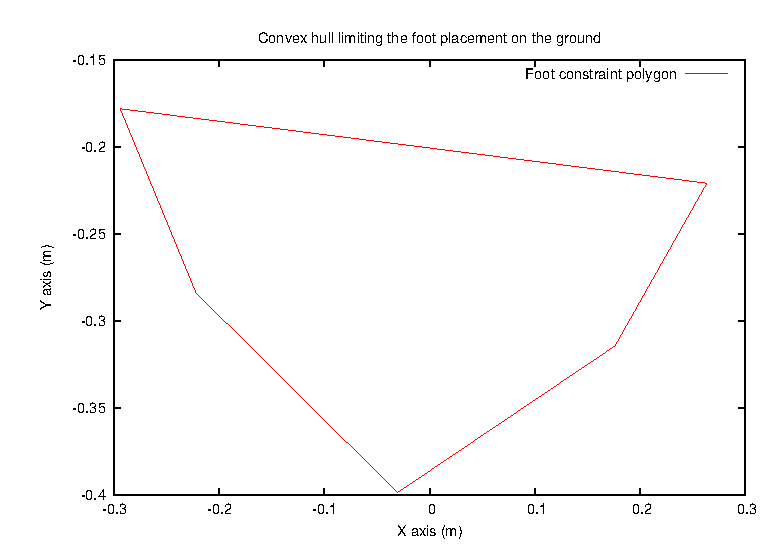
\includegraphics[width=15cm]{./figures/walking-without-thinking/ConvexHull}
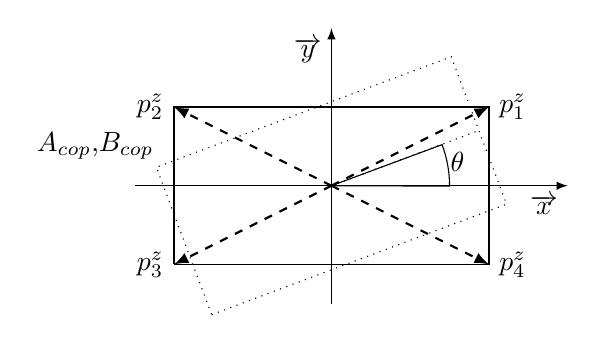
\begin{tikzpicture}[scale=0.050, node distance=2cm,>=latex]
\draw [->](-50,0) -- (60,0) node [below left, black]{$\overrightarrow{x}$}; %x-axis
\draw [->](0,-30) -- (0,40) node [below left, black]{$\overrightarrow{y}$}; %y-axis
 %support foot
\draw (-40,-20)--(40,-20)--(40,20)--(-40,20)--(-40,-20);

\draw [thick][dashed][->](0,0) -- (40,20) node [right, black]{${p}^z_1$}; %y-axis
\draw [thick][dashed][->](0,0) -- (-40,20) node [left, black]{${p}^z_2$}; %y-axis
\draw [thick][dashed][->](0,0) -- (-40,-20) node [left, black]{${p}^z_3$}; %y-axis
\draw [thick][dashed][->](0,0) -- (40,-20) node [right, black]{${p}^z_4$}; %y-axis
\draw node at (-60,10) {$A_{cop}$,$B_{cop}$}; %y-axis

% rotated support foot
\draw [dotted][cm={cos(\tetazero) ,sin(\tetazero) ,-sin(\tetazero) ,cos(\tetazero) ,(0.0 cm,0.0 cm)}]
(-40,-20)--(40,-20)--(40,20)--(-40,20)--(-40,-20) ;
% rotated axis
\draw [dotted][-][cm={cos(\tetazero) ,sin(\tetazero) ,-sin(\tetazero) ,cos(\tetazero) ,(0.0 cm,0.0 cm)}]
(0,0) -- (40,0) node [below left, black]{};
% angle
\draw (0,0) -- (28.090986571,10.432619456) arc (\tetazero:0:30) -- (0.0,0.0) node at (32,6) {$\theta$} ;

\end{tikzpicture}
}
    \caption[Balance constraint]{Shape of the foot with the position vector $ {p}^z_{i} $ describing the support polygon and $ \theta $ representing its orientation.
    The $4\times2$ matrix $A_{cop}$ and the $4\times1$ vector $B_{cop}$ are the linear algebra representation of the edges.}
	\label{fig:foot}
\end{figure}

The CoP has to remain inside the support polygon \cite{Wieber:IWFFFR:2002}.
This polygon is depicted in Fig.~\ref{fig:foot}.
The set of linear inequalities representing the convex polygon is denoted as $A_{cop}$ and $B_{cop}$.
Only one foot is modeled as a support polygon for two reasons:
1) HRP-2 feet are symmetrical, 2) the sampling period of the problem is designed in a way that no iteration of the optimization problem falls into a double support phase.
The CoP at instant $k$, \mbox{($z_k = [z_k^x \;\; z_k^y]^T$)}, see Sec.~\ref{SubSec:LIPM}) lies inside the support polygon if and only if
\begin{align}
  A_{cop} R(f_k^\theta) \left( {z}_k - f_k
  \right) \leq B_{cop} \\
  \left[A_{cop,k}^{x,\theta} \;\;\;\;  A_{cop,k}^{y,\theta} \right] \left( {z}_k - f_k
  \right) \leq B_{cop} \\
  R(f_k^{\theta} ) =
  \begin{bmatrix}
  \cos(f_k^\theta) & \sin(f_k^\theta)\\
  -\sin(f_k^\theta) & \cos(f_k^\theta)
  \end{bmatrix}
  ,
\end{align}
where $f_k = [f_k^x \;\; f_k^y]^T$, $A_{cop,k}^{x,\theta}$ is the left column of $A_{cop} R(f_k^\theta)$ and $A_{cop,k}^{y,\theta}$ is the right one.
Using eq.~\eqref{eq:Fkp1} the constraint for each time step of the preview horizon is defined by
\begin{equation}
\label{eq:cop_constraint_extended}
D_{k+1}(U_k^\theta)
\begin{bmatrix}
Z_{k+1}^x - v_{k+1} f_{k}^x - V_{k+1} \tilde{F}_{k+1}^x \\
Z_{k+1}^y - v_{k+1} f_{k}^y - V_{k+1} \tilde{F}_{k+1}^y
\end{bmatrix} \leq
b_{cop}\,_{k+1}
\end{equation}
With $b_{cop}\,_{k+1} = [B_{cop} \hdots B_{cop}]^T$ and $D_{k+1}(U_k^\theta) = $
\begin{equation*}
\begin{bmatrix}
A_{cop,k+1}^{x,\theta} & & 0 & A_{cop,k+1}^{y,\theta} & & 0 \\
 & \ddots & & & \ddots \\
0 & & A_{cop,k+N}^{x,\theta} & 0 & & A_{cop,k+N}^{y,\theta} \\
\end{bmatrix}
.
\end{equation*}
From eq.~(\ref{eq:cop_constraint_extended}), the canonical form of the constraint is
\begin{equation}
A_{cop,k}(U_k^\theta) \; U^{x,y}_{k} \;\leq\; \overline{U_{cop,k}}
,
\label{eq:zmpCanonicConstraint}
\end{equation}
where $A_{cop,k}(U_k^\theta)$ is a matrix depending on $ U_k^\theta $ which makes this constraint nonlinear.
And $\overline{U_{cop,k}}$ is the upper bound vector. %symbolized with the over line.
The last steps of the derivation are detailed in \cite{herdt:iros:2010}.

\begin{figure}[ht]
    \centering
    %!TEX root = ../../NMPC_WPG.tex

\newcommand{\tetazero}{20.55}
\newcommand{\Fkxzero}{-20}
\newcommand{\Fkyzero}{20}

\newcommand{\tetaone}{-20}
\newcommand{\Fkxone}{5}
\newcommand{\Fkyone}{0}

\newcommand{\tetatwo}{20}
\newcommand{\Fkxtwo}{25}
\newcommand{\Fkytwo}{20}

%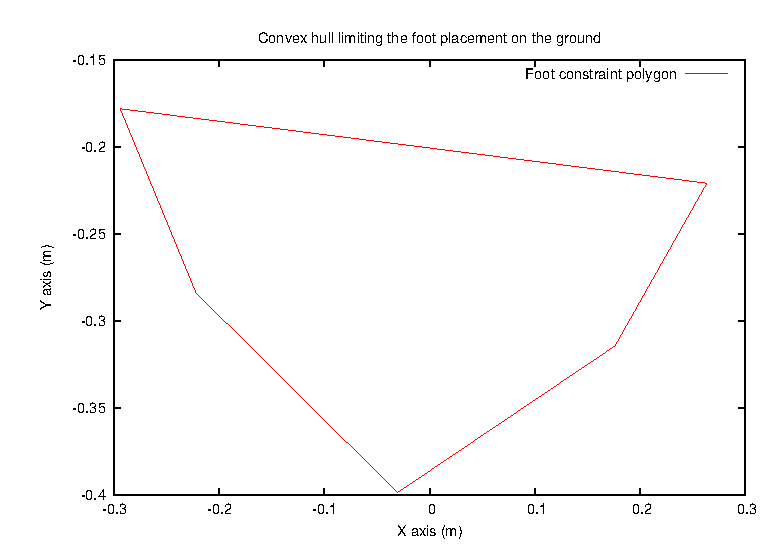
\includegraphics[width=15cm]{./figures/walking-without-thinking/ConvexHull}
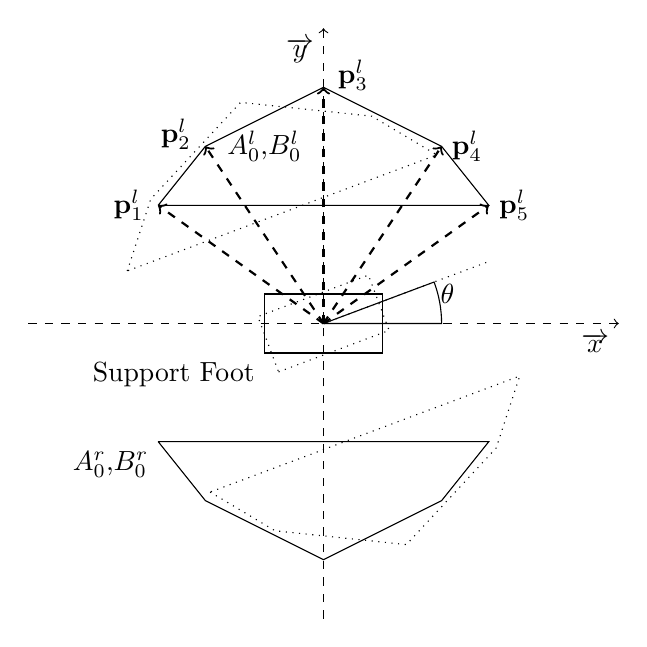
\begin{tikzpicture}[scale=0.075]
\draw [dashed][->](-50,0) -- (50,0) node [below left, black]{$\overrightarrow{x}$}; %x-axis
\draw [dashed][->](0,-50) -- (0,50) node [below left, black]{$\overrightarrow{y}$}; %y-axis
 %right support, left foot landing convexhull
\draw (-28,-20)--(-20,-30)--(0,-40)--(20,-30)--(28,-20)--(-28,-20) node [below left, black]{$A^r_0$,$B^r_0$} ;
 %left support, right foot landing convexhull
\draw (-28,20)--(-20,30)--(0,40)--(20,30)--(28,20)--(-28,20) node at (-10,30)[black]{$A^l_0$,$B^l_0$} ;
 %support foot
\draw (-10,-5)--(10,-5)--(10,5)--(-10,5)--(-10,-5) node [below left, black]{Support Foot} ;

% rotated support foot
\draw [dotted][cm={cos(\tetazero) ,sin(\tetazero) ,-sin(\tetazero) ,cos(\tetazero) ,(0.0 cm,0.0 cm)}]
(-10,-5)--(10,-5)--(10,5)--(-10,5)--(-10,-5) ;
% rotated axis
\draw [dotted][-][cm={cos(\tetazero) ,sin(\tetazero) ,-sin(\tetazero) ,cos(\tetazero) ,(0.0 cm,0.0 cm)}]
(0,0) -- (30,0) node [below left, black]{};
% angle
\draw (0,0) -- (18.727324381,7.02049297) arc (\tetazero:0:20) -- (0.0,0.0) node at (21,5) {$\theta$} ;
% rotated left support, right foot landing convexhull
\draw [dotted][-][cm={cos(\tetazero) ,sin(\tetazero) ,-sin(\tetazero) ,cos(\tetazero) ,(0.0 cm,0.0 cm)}]
(-28,20)--(-20,30)--(0,40)--(20,30)--(28,20)--(-28,20) ;
% rotated right support, left foot landing convexhull
\draw [dotted][-][cm={cos(\tetazero) ,sin(\tetazero) ,-sin(\tetazero) ,cos(\tetazero) ,(0.0 cm,0.0 cm)}]
(-28,-20)--(-20,-30)--(0,-40)--(20,-30)--(28,-20)--(-28,-20);

\draw [thick][dashed][->](0,0) -- (-28,20) node [black] at (-33.0,20.0){${\bf p}_1^l$}; %y-axis
\draw [thick][dashed][->](0,0) -- (-20,30) node [black] at (-25.0,32.0){${\bf p}_2^l$}; %y-axis
\draw [thick][dashed][->](0,0) -- (0.0,40) node [black] at (5.0,42.0){${\bf p}_3^l$}; %y-axis
\draw [thick][dashed][->](0,0) -- (20,30) node [right, black]{${\bf p}_4^l$}; %y-axis
\draw [thick][dashed][->](0,0) -- (28,20) node [right, black]{${\bf p}_5^l$}; %y-axis

\end{tikzpicture}

    \caption[Foot position constraint]{Shape of the selected convex polygon boundary of the foot placement. The $5\times2$ matrix $A_\textup{r,l}$ and the $5\times1$ vector $B_\textup{r,l}$, define the convex hull as a set of linear inequalities.}
	\label{fig:convexHull}
\end{figure}

\subsubsection{Foot step feasibility constraint}
\label{Sec:constraintOnFootPlacement}

This constraint uses the same convex hull as in \cite{herdt:iros:2010} to ensure the feasibility of the steps \cite{perrin2010approximation}.
For HRP-2 this convex hull is shown in Fig.~\ref{fig:convexHull}.
The set of linear inequalities representing this convex polygon is defined by $A_{foot}$ and $B_{foot}$.
Instead of $r$ or $l$ the lower index $foot$ is used because the problem is symmetrical.
The constraint, representing the fact that the swing foot has to land inside the convex hull, is given as
\begin{equation}
A_{foot} R(\theta) ({f}_{k+1} - {f}_k ) \leq B_{r,l}
.
\end{equation}
In the exact manner as in eq.~\eqref{eq:zmpCanonicConstraint}, the vector and matrices depicted in Sec.~\ref{Sec:dynamic} are used to express this constraint for each previewed foot step.
More details are presented in \cite{herdt:iros:2010}.
The canonical form of the constraint is
\begin{equation}
A_{foot,k}(U^\theta_k) \; U^{x,y}_{k} \;\leq\; \overline{U_{foot,k}}
,
\label{eq:footCanonicConstraint}
\end{equation}

where $A_{foot,k}(U^\theta_k)$ depends on $U_k^{\theta}$ like $A_{cop,k}(U_k^\theta)$, which makes this constraint nonlinear.
And $\overline{U_{foot,k}}$ is the upper bound vector.% symbolized with the over line.


\subsubsection{Foot orientation constraint}
\label{Sec:constraintOnFootOrientation}

One additional feasibility constraint considers the maximum and minimum angle between both feet
\begin{equation}
    -\theta_{thresh} \leq F_{k+1}^\theta - F_{k}^\theta \leq \theta_{thresh} \label{eq:ori_constraint}
    ,
\end{equation}
with the canonical form
\begin{align}
    \underline{U_{\theta,k}} &\leq A_{\theta} U_k^\theta \leq \overline{U_{\theta,k}} \\
    \label{eq:thetaCanonicConstraint}
\text{with : }    A_{\theta} &=
    \begin{bmatrix}
    		 1 &  0 & 0 & 0 \\
    		-1 &  1 & \ddots & \vdots \\
      	 0 & \ddots & \ddots & 0  \\
    		 \ddots & 0 & -1 & 1
    	\end{bmatrix}, \nonumber\\
    \overline{U_{\theta,k}} &=
    	\begin{bmatrix}
    		 \theta_{thresh} + f_k^{\theta} & &
    		 \theta_{thresh} &
    		 \hdots &
    		 \theta_{thresh}
    	\end{bmatrix}^T , \nonumber \\
    \underline{U_{\theta,k}} &=
    	\begin{bmatrix}
    		 -\theta_{thresh} + f_k^{\theta} & &
    		 -\theta_{thresh} &
    		 \hdots &
    		 -\theta_{thresh}
    	\end{bmatrix}^T \nonumber
        .
\end{align}
In practice the bound $\theta_{thresh} = 0.05rad$ takes into account the hardware limits.
At this stage, the optimization problem allows the robot to place its feet anywhere inside the convex hull at any moment.
In \cite{herdt:iros:2010}, the velocity of the foot is limited by bounding the feasible foot step area that corresponds to a maximum velocity.
We chose to use the same idea extended to all the foot steps degrees of freedom.
This significantly decreases the variation of accelerations before foot landing.

\subsection{Additional constraint : local obstacle avoidance}
\label{Sec:avoidAnObstacle}

% Let us now derive the local obstacle avoidance constraint.
Here, only the convex obstacles are considered. For simplification the obstacle is defined as a circle $ C = $~$\{ (p^x,p^y) \in $~$\mathcal{R}^2, (p^x-x_0)^2+(p^y-y_0)^2 = R^2\}$
Where $x_0$ and $y_0$ are its center coordinates in the world frame and $R$ its radius.
The previewed foot steps are feasible if they are outside the circle.
This constraint does not depend on the orientation of the foot steps.
For the $j^{th}$ previewed step, at iteration $k+j$ the constraint is expressed by
\begin{align}
\left(f_{k+j}^x - x_0 \right)^2 + \left(f_{k+j}^y - y_0 \right)^2 \geq R^2 + m^2 \\
\iff \;\; U_k^T H_{obs,j} U_k + A_{obs,j} U_k \;\geq \underline{U_{obs,j}} \;\;\;\;\;
,
\end{align}
with $H_{obs,j}$ a selection matrix, $A_{obs,j}$ a vector depending on $x_0$ and $y_0$, and $m$ a security margin taking into account the swept volume of the robot.

\subsection{The solver}
\label{sec:linearization}
This paragraph presents the method used to solve the problem detailed in the previous sections.
The non-linearity of the constraint and the still quadratic objective classifies the former LQR scheme as a nonlinear least squares optimization problem, which has the general form
\begin{subequations}
    \label{eq:nonlinear_problem}
    \begin{align}
        \min_{U_k}  \quad & \frac{1}{2} \lVert l(U_k) \rVert_2^2 \label{eq:nonlinear_problem_objective}\\
        \text{s.t.} \quad & \underline{h} \leq h(U_k) \leq \overline{h} \label{eq:nonlinear_problem_constraints}.
    \end{align}
\end{subequations}
In general, derivative-based methods in the form of sequential quadratic programming~{SQP} can be used for nonlinear optimization problems.
These methods are called SQP because at each iteration a second order approximation of the nonlinear problem is calculated.
Here, the least squares structure can be exploited to solve eq.~\eqref{eq:nonlinear_problem} more efficiently using a generalized Gau\ss-Newton method.
Starting with an initial guess $U_{k-1}$ the method iterates $U_{k} = U_{k-1} \,+\, \Delta U_k$,
where the increment $\Delta U_k$ is obtained from the solution of the following QP approximation under the following form
\begin{subequations}
    \label{eq:second_order_approximation}
    \begin{align}
        \min_{\Delta U_k} \quad & \frac{1}{2} \lVert l_{k-1} + (\nabla_{U_{k}} l_k|_{U_{k-1}})^T \Delta U_k \rVert_2^2 \label{eq:second_order_approximation_objective}\\
        \text{s.t.} \quad & \underline{h} - h_{k-1} \leq (\nabla_{U_{k}} h_k|_{U_{k-1}})^T \Delta U_k \leq \overline{h} - h_{k-1}
        \label{eq:second_order_approximation_inequality_constraints}
    \end{align}
\end{subequations}
with
\begin{equation*}
    l_k := l(U_k),\ h_k := h(U_k) \,.
\end{equation*}
Reformulating eq.~\eqref{eq:second_order_approximation} as a QP in canonical form, we get
\begin{subequations}
    \label{eq:final_qp}
    \begin{align}
        \min_{\Delta U_k} \quad & \frac{1}{2} \Delta U_{k}\,^T \tilde{Q_k} \Delta U_{k} + \tilde{p_k}^T \Delta U_{k} \\
        \text{s.t.}       \quad & \underline{\tilde{U_k}} \leq \tilde{A_k} \Delta U_k \leq \overline{\tilde{U_k}}
    \end{align}
\end{subequations}
with
\begin{align}
    \label{eq:problem_objective}
    \tilde{Q_k} &= Q_k
    ,\;\;\;\;
    \tilde{p_k} =
    \begin{bmatrix}
        \frac{1}{2} (U_{k-1}^{x,y})^T Q_k^{x,y}       + p_k^{x,y} \\
        \frac{1}{2} (U_{k-1}^{\theta})^T Q_k^{\theta} + p_k^{\theta}
    \end{bmatrix} \notag \\
    \tilde{A_k} &=
    \begin{bmatrix}
A_{cop,k}(U_{k-1}^\theta) &
\nabla_{U_{k}^{\theta}}^T A_{cop,k}|_{U_{k-1}^\theta} \; U_{k-1}^{x,y}\\
A_{foot,k}(U_{k-1}^\theta)&
\nabla_{U_{k}^{\theta}}^T A_{foot,k}|_{U_{k-1}^\theta} \; U_{k-1}^{x,y}\\
0 & A_{\theta} \\
H_{obs,j} U_{k-1} + A_{obs,j} &   0
    \end{bmatrix}, \notag
    \\
    \underline{\tilde{U_k}} &=
    \begin{bmatrix}
        -\infty \\
        -\infty \\
        \underline{U_{\theta,k}}\\
        \underline{U_{obs,j}}
    \end{bmatrix}
    - h_{k-1} \;,\;\;\;\;\;\;
    \overline{\tilde{U_k}} =
    \begin{bmatrix}
        \overline{U_{cop,k}} \\
        \overline{U_{foot,k}} \\
        \overline{U_{\theta,k}} \\
        +\infty
    \end{bmatrix}
    - h_{k-1} \;, \notag \\
    h_{k-1} &=
    \begin{bmatrix}
        A_{cop,k}(U_{k-1}^\theta) \; U_{k-1}^{x,y} \\
        A_{foot,k}(U_{k-1}^\theta) \; U_{k-1}^{x,y} \\
        A_{\theta} \; U_{k-1}^{\theta} \\
        U_{k-1}^T H_{obs,j} U_{k-1} + A_{obs,j} U_{k-1}
    \end{bmatrix} \; , \; \notag \\
    &\forall j \in {1, \hdots , nf} \notag
    .
\end{align}
In this work the NMPC scheme is based on the idea of the so called "real-time iteration" \cite{bock_numerical_2007,diehl_real-time_2002}.
At each time instant of the control loop the nonlinear problem resolution requires the use of a SQP method.
However by carefully initializing the applied SQP method and by preserving the state from the last iteration, the computational effort can be reduced to solving a single QP (one iteration of the respective SQP method) at each time. Furthermore, the computational process can be separated into three phases, two of which can be completed in advance without knowledge of the actual process state. In this way, the feedback delay can be drastically reduced.
Therefore, instead of solving eq.~\eqref{eq:nonlinear_problem} we recalculate its linearization once at each iteration of the control loop and solve a single QP eq.~\eqref{eq:final_qp} in each iteration.
This allows a real-time execution on the robot even for the proposed nonlinear formulation.

\subsection{The line search}
\label{sec:linesearch}

From experiments, we never found optimal solution of the linearized problem that did not satisfy the nonlinear problem constraints.
However to decrease the time consumption of the algorithm we limited the maximum time and active set recalculation of the solver.
In that case, the solver provides a sub-optimal solution which does not necessarily satisfy the constraint of the original problem.
The classical approach, in that case, is to use a line search.
It basically consists in finding a scalar $s$ which scales the found solution:
\begin{equation}
U_k = U_{k-1} + s \Delta U_k
\label{equ:uks}
\end{equation}
The idea is to choose $s:=1$ for a start and verify the constraints using $U_k$.
If the constraints are not verified we decrease $s:=0.6s$ and we update $U_k$ using \ref{equ:uks}.
The algorithm check the constraints using the updated $U_k$ and decrease again $s$ if needed.
The algorithm end if $s$ is too small or if the constraints are verified.
This way we verify that the constraint are verified and that the solver does not take more than the allocated time to find a solution.
